\documentclass[aspectratio=169,11pt]{beamer}
\usetheme{default}
\usecolortheme{whale}
\setbeamertemplate{navigation symbols}{}
\setbeamertemplate{footline}{%
  \hbox{\begin{beamercolorbox}[wd=\paperwidth,ht=2.2ex,dp=1ex,leftskip=1.2em,rightskip=1.2em]{author in head/foot}%
    \tiny\itshape S\textsuperscript{4}D: state-of-the-art hierarchical speculative decoding\hfill\upshape\insertframenumber\,/\,\inserttotalframenumber%
  \end{beamercolorbox}}%
}
\setbeamerfont{frametitle}{series=\bfseries}
\setbeamercolor{frametitle}{fg=white,bg=structure}
\usepackage{graphicx}
\usepackage{tikz}
\usetikzlibrary{arrows.meta,positioning}
\usepackage{amsmath}
\usepackage{booktabs}
\usepackage{colortbl}
\setbeamertemplate{itemize items}[circle]
\setbeamertemplate{note page}{\insertnote}

\setbeameroption{show notes}

\title{\textbf{S\textsuperscript{4}D}}
\author{Nicole Ma \and Harsh Singh}
\date{}

\begin{document}

\begin{frame}\titlepage\end{frame}
\note{
We're Nicole and Harsh, presenting S-four-D, a new state-of-the-art method for hierarchical speculative decoding.
}

% =====================================================================
\begin{frame}{Overview}
\textbf{We introduce the first reinforcement-learned routing policy for hierarchical speculative decoding, and set a new state of the art.}
\vspace{6pt}

{\footnotesize VIA-SD adds a slim intermediate verifier, but routes between tiers using confidence thresholds tuned by hand.}
\vspace{4pt}

We present \textbf{three key contributions}:
\begin{enumerate}
  \item A \textbf{learned per-token gating policy} that recasts tier-routing as a sequential decision problem, so a tiny $q$-free MLP replaces the fixed thresholds.
  \item A \textbf{reward} that balances output quality against the latency of expensive verifier calls.
  \item A \textbf{per-token RL formulation} with principled credit assignment (REINFORCE, then GRPO, then a per-token advantage).
\end{enumerate}
\vspace{2pt}
{\footnotesize\textbf{The payoff:} we match \emph{lossless} accuracy (\textbf{0.91}) at \textbf{4$\times$ fewer} full-model calls,
\textbf{2.2$\times$} faster than greedy. We \textbf{Pareto-dominate} the paper's VIA-SD at roughly \textbf{2$\times$ its speedup and 2.3$\times$ its accuracy},
and reach up to \textbf{3.5$\times$} when pushed for speed.}
\end{frame}
\note{
Speculative decoding speeds up LLMs. VIA-SD adds a slim middle verifier but routes with hand-tuned thresholds. Our three contributions: a learned per-token gate, a quality-versus-cost reward, and per-token RL. The payoff: lossless accuracy at four times fewer calls, up to three and a half times faster, a new state of the art.
}

% =====================================================================
\begin{frame}{The bottleneck: LLM decoding is slow and sequential}
\begin{itemize}
  \item Generating each token streams the entire model from memory, so LLM inference is memory-bandwidth bound and dominated by sequential forward passes.
  \item Speculative decoding fixes this: a cheap \emph{drafter} guesses several tokens, and the big \emph{verifier} checks them all in one parallel pass.
  \item Accepted guesses give many tokens per expensive forward. It is \textbf{lossless}, and runs about \textbf{1.4$\times$} faster on our models.
  \item The one lever is the \textbf{acceptance rate}, because every rejected token forces a full-model step.
\end{itemize}
\end{frame}
\note{
Each token streams the whole model from memory, so inference is slow. Speculative decoding lets a small drafter guess and the big model verify in parallel: lossless, about 1.4 times faster. The lever is the acceptance rate.
}

% =====================================================================
\begin{frame}{VIA-SD improves on vanilla SD}
\begin{columns}
\begin{column}{0.56\textwidth}
Vanilla SD makes a \textbf{binary} choice per token: accept the drafter, or reject and pay for the full model $q$.
\vspace{5pt}

VIA-SD adds a \textbf{slim middle verifier $q'$} (the target $q$ with about 45\% of its layers skipped), giving \textbf{three} choices.
Borderline ``middle-zone'' tokens are handled cheaply by $q'$, so the full model is called far less often.
\vspace{4pt}

{\footnotesize Since $q'$ is the target verifying its \emph{own} draft through a reduced copy of itself, this is the \textbf{Semi-Self} in S\textsuperscript{4}D.}
\end{column}
\begin{column}{0.44\textwidth}
\centering
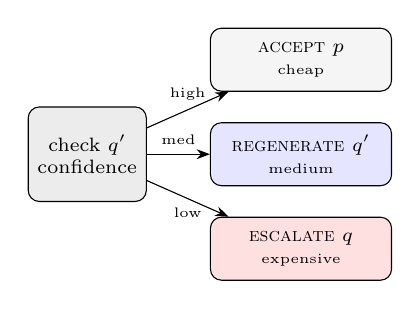
\begin{tikzpicture}[font=\scriptsize,>=Stealth,
  m/.style={draw,rounded corners,minimum width=23mm,minimum height=8mm,align=center},
  d/.style={draw,fill=gray!15,rounded corners,align=center,minimum height=12mm,minimum width=15mm}]
\node[d] (dec) {check $q'$\\confidence};
\node[m,fill=gray!8,right=8mm of dec,yshift=12mm] (a) {\textsc{accept} $p$\\\tiny cheap};
\node[m,fill=blue!10,right=8mm of dec] (r) {\textsc{regenerate} $q'$\\\tiny medium};
\node[m,fill=red!12,right=8mm of dec,yshift=-12mm] (e) {\textsc{escalate} $q$\\\tiny expensive};
\draw[->](dec)--(a) node[midway,above,font=\tiny]{high};
\draw[->](dec)--(r) node[midway,above,font=\tiny]{med};
\draw[->](dec)--(e) node[midway,below,font=\tiny]{low};
\end{tikzpicture}
\end{column}
\end{columns}
\end{frame}
\note{
VIA-SD adds a slim middle verifier, the target with half its layers skipped, giving three choices: accept, regenerate, or escalate. Borderline tokens go to the cheap tier. Because the model verifies its own draft through a reduced copy of itself, that is the Semi-Self in our name.
}

% =====================================================================
\begin{frame}{But it routes with thresholds that are picked by hand}
VIA-SD makes the three-way choice with \textbf{two fixed confidence thresholds} on $q'$:
\quad $\boxed{\alpha_1 = 0.5}$ \quad $\boxed{\alpha_2 = 0.3}$.
\vspace{4pt}
\begin{itemize}
  \item They are \textbf{global and static}: one cutoff for every token and every context.
  \item They are \textbf{brittle}, and must be re-tuned for each new model and task.
  \item They are \textbf{sub-optimal}: even after a full sweep, accuracy peaks at $0.50$ on our setup.
\end{itemize}
\vspace{4pt}
Choosing a tier for each token, from its context, is a sequential decision problem. \textbf{So we learn it} --- the gate teaches itself. That is the \textbf{Self-Taught} in S\textsuperscript{4}D.
\end{frame}
\note{
But VIA-SD picks between tiers with two hand-tuned thresholds, 0.5 and 0.3. They're global, brittle, and cap at 0.50 accuracy even fully swept, because one cutoff can't adapt to context. Routing per token is a decision problem, so the gate teaches itself: the Self-Taught.
}

% =====================================================================
\section{Method}
\begin{frame}{Contribution 1/3: a learned per-token gating policy (MDP)}
\begin{columns}
\begin{column}{0.56\textwidth}
\small We recast tier-routing as a \textbf{Markov decision process}:
\begin{itemize}
  \item \textbf{State} $s_t$: $q$-free features (drafter/$q'$ confidence, agreement, $\mathrm{KL}(p\Vert q')$, position).
  \item \textbf{Action} $a_t\in\{$accept, regenerate, escalate$\}$.
  \item \textbf{Policy} $\pi_\theta(a_t\mid s_t)$: a tiny MLP.
\end{itemize}
\vspace{3pt}
\footnotesize The full model $q$ is consulted only to \emph{score} at train time. It is never a gate input,
so the gate is free to run at inference.
\end{column}
\begin{column}{0.44\textwidth}
\centering
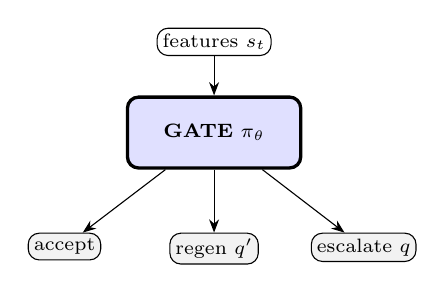
\begin{tikzpicture}[font=\scriptsize,>=Stealth,
  g/.style={draw,very thick,fill=blue!12,rounded corners,minimum width=22mm,minimum height=9mm,align=center},
  a/.style={draw,rounded corners,fill=gray!10,align=center,inner sep=2pt},
  io/.style={draw,rounded corners,align=center,inner sep=2pt}]
\node[io] (f) {features $s_t$};
\node[g,below=5mm of f] (g) {\textbf{GATE} $\pi_\theta$};
\node[a,below=8mm of g,xshift=-19mm] (x){accept};
\node[a,below=8mm of g] (y){regen $q'$};
\node[a,below=8mm of g,xshift=19mm] (z){escalate $q$};
\draw[->](f)--(g);\draw[->](g)--(x);\draw[->](g)--(y);\draw[->](g)--(z);
\end{tikzpicture}
\end{column}
\end{columns}
\end{frame}
\note{
Contribution one: the learned gate, framed as an MDP. State is cheap q-free features, action is the tier, policy is a tiny MLP. The full model is used only for rewards at training time, never to decide, so the gate is free to deploy.
}

% =====================================================================
\begin{frame}{Contribution 2/3: a reward balancing quality and cost}
\textbf{Two ingredients per token:}
\begin{align*}
\text{quality:}\quad & \text{match}_t = \mathbf{1}\big[\hat y_t = \arg\max\nolimits_v q(v\mid x_{<t})\big] \\[-1pt]
\text{cost:}\quad & \text{cost}_t = \big(t_{p_1} + t_{q'}/\gamma + \mathbf{1}[\textsc{escalate}]\,t_q\big)\big/\,t_{q_1}
\end{align*}
\textbf{Reward} (cost in units of one full-model step):
\begin{align*}
\text{trajectory:}\ & R = \overline{\text{match}} - \lambda\,\overline{\text{cost}}\ (+\,r_c\,\text{correct})
\qquad\qquad
\text{per-token:}\ r_t = \text{match}_t - \lambda\,\text{cost}_t
\end{align*}
\centering\footnotesize $\lambda$ is the quality-versus-speed knob. \texttt{match} is a \emph{dense} proxy for the
sparse true objective (final-answer correctness).
\end{frame}
\note{
Contribution two: the reward, match minus lambda times cost. Quality is whether our token matches the full model; lambda trades accuracy for speed. One caveat: match is a proxy, and ninety-eight percent token match still gives only 0.72 final accuracy, because slips compound.
}

% =====================================================================
\begin{frame}{Contribution 3/3: per-token RL with credit assignment}
\textbf{Policy gradient} (all variants, plus an entropy bonus $\eta\,\mathcal{H}[\pi_\theta]$):
\[
\nabla_\theta J = \mathbb{E}\Big[\textstyle\sum_t A_t\,\nabla_\theta \log \pi_\theta(a_t\mid s_t)\Big]
\]
They differ only in the \textbf{advantage} $A_t$:
\begin{itemize}\small
  \item \textbf{REINFORCE} (trajectory): $A = R - b$, with EMA baseline $b\leftarrow(1{-}\tau)b+\tau R$.
  \item \textbf{GRPO} (group): $A_i = \dfrac{R_i-\mathrm{mean}_{\mathcal G}R}{\mathrm{std}_{\mathcal G}R}$, with PPO-clip $\rho_t=\frac{\pi_\theta}{\pi_{\theta_{\text{old}}}}$ and KL to $\pi_{\text{ref}}$.
  \item \textbf{per-token (v2):} $\hat A_t = \dfrac{r_t-\mathrm{mean}_{\text{batch}}\,r}{\mathrm{std}_{\text{batch}}\,r}$, local credit and the \textbf{lowest variance}.
\end{itemize}
\end{frame}
\note{
Contribution three: per-token RL. Same policy gradient; they differ only in the advantage. REINFORCE uses one noisy trajectory reward, GRPO normalizes within a group, and our per-token version gives each decision its own advantage: lowest variance, best results. Credit assignment is everything.
}

% =====================================================================
\section{Results}
\begin{frame}{Training converges, and per-token (v2) is cleanest}
\centering
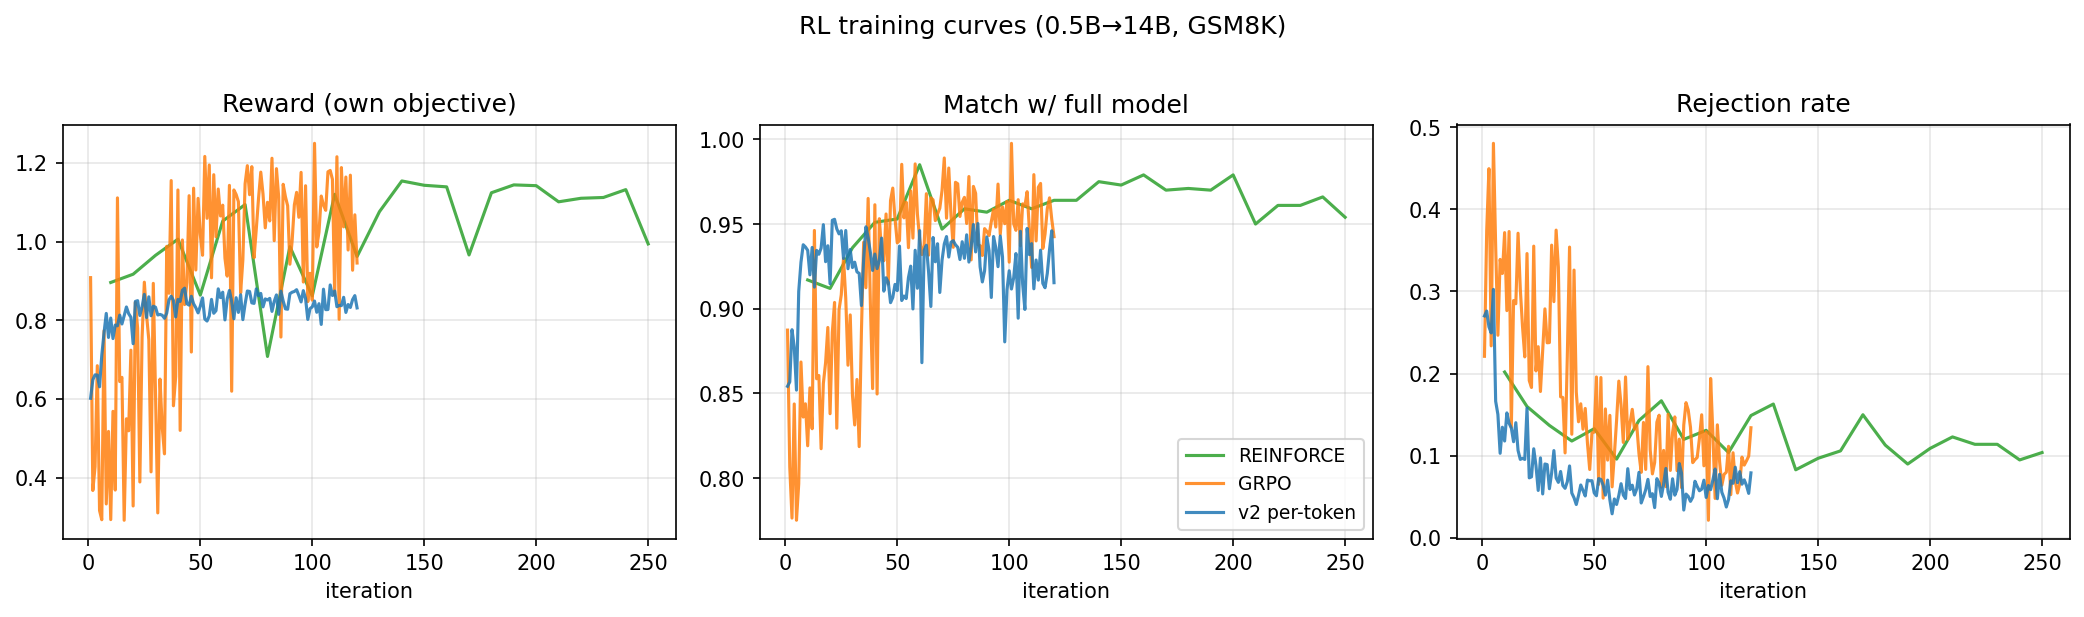
\includegraphics[width=0.9\textwidth]{results/figures/rl_curves.png}
\end{frame}
\note{
All three converge, match reaches about 0.95, rejection falls, and per-token in blue is smoothest. Match plateaus at 0.95, not 1.0, and that residual is what compounds into the accuracy gap.
}

% =====================================================================
\begin{frame}{Results: the learned gate dominates}
\centering\small
\begin{tabular}{lccc}
\toprule
Method & GSM8K acc & q-calls/tok & speedup \\
\midrule
greedy-$q$ (reference)        & 0.887 & 1.000 & 1.00$\times$ \\
plain SD (standard, lossless) & 0.907 & 0.259 & 1.40$\times$ \\
\midrule
\rowcolor{red!8} via\_fixed (paper, tuned)  & 0.40 & 0.31 & 1.76$\times$ \\
\rowcolor{red!8} via\_imit (imitation only) & 0.34 & 0.29 & 1.69$\times$ \\
\midrule
\rowcolor{blue!8} via\_rl REINFORCE          & 0.880 & 0.243 & 2.29$\times$ \\
\rowcolor{blue!8} via\_rl GRPO               & 0.853 & \textbf{0.162} & 2.94$\times$ \\
\rowcolor{blue!8} via\_rl REINFORCE+DIMR     & \textbf{0.907} & 0.250 & 2.22$\times$ \\
\rowcolor{blue!8} via\_rl v2 per-token       & 0.713 & 0.104 & \textbf{3.53$\times$} \\
\bottomrule
\end{tabular}
\vspace{3pt}
\centering\structure{\textbf{$\Rightarrow$ S\textsuperscript{4}D is state-of-the-art hierarchical speculative decoding.}}
\end{frame}
\note{
The numbers. The hand-tuned thresholds, in red, are broken at 0.34 to 0.40: the slim verifier is miscalibrated, so a global cutoff can't tell confident-correct from confident-wrong, and errors compound. Our learned gates, in blue, recover full lossless accuracy, 0.907. This is state-of-the-art hierarchical speculative decoding.
}

% =====================================================================
\begin{frame}{Latency: speedup by method}
\centering
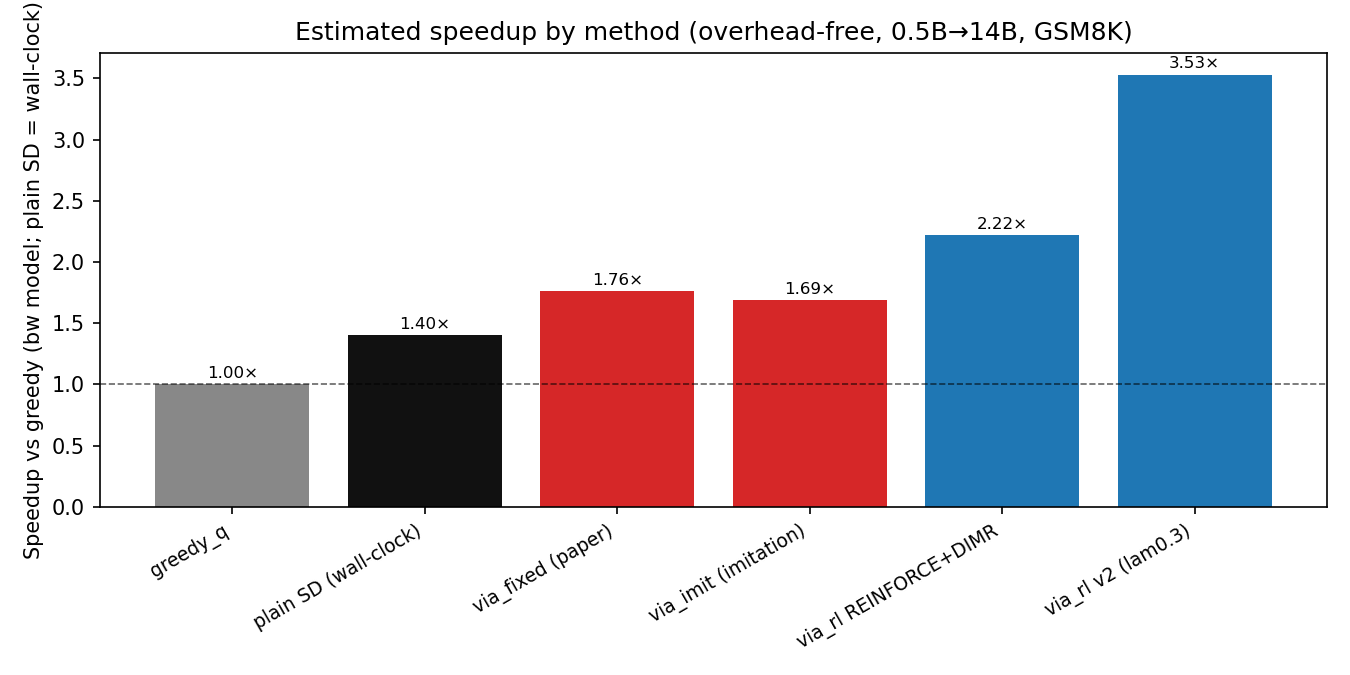
\includegraphics[width=0.8\textwidth]{results/figures/speedup_bar.png}
\end{frame}
\note{
Latency. The hand-tuned gate is slow because it over-escalates. Our learned gates are fastest, with per-token on top.
}

% =====================================================================
\begin{frame}{The accuracy and speed frontier}
\centering
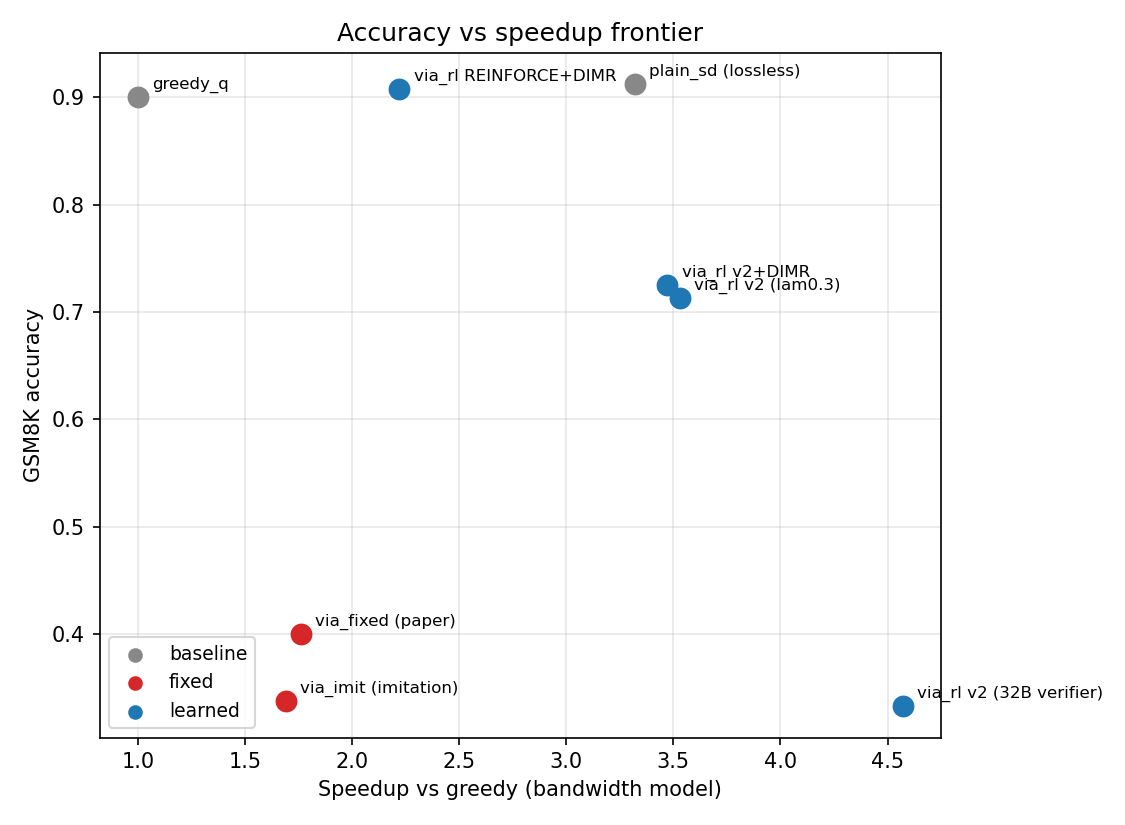
\includegraphics[width=0.6\textwidth]{results/figures/pareto.png}
\end{frame}
\note{
Accuracy versus speed. Red is dominated on both axes, because one cutoff can't both avoid over-escalating and avoid over-accepting. Blue, our learned gates, dominate, with a full frontier from lambda. We Pareto-dominate the baseline, which makes S4D state of the art.
}

% =====================================================================
\begin{frame}{Ablation: which model should we scale?}
\centering\small
\begin{tabular}{lccl}
\toprule
Setup & GSM8K acc & q-calls/tok & note \\
\midrule
0.5B $\to$ 14B (main) & 0.88--0.91 & 0.10--0.25 & baseline pair \\
\rowcolor{green!10} \textbf{3B} $\to$ 14B \;(bigger \emph{drafter}) & 0.80 & \textbf{0.028} & \textbf{36$\times$ fewer} full-model calls \\
\rowcolor{red!10} 0.5B $\to$ \textbf{32B} \;(bigger \emph{verifier}) & \textbf{0.33} & 0.07 & accuracy collapses \\
\bottomrule
\end{tabular}
\vspace{4pt}
\begin{itemize}\small
  \item A stronger \textbf{drafter} raises acceptance, so the gate escalates far less at similar accuracy.
  \item A bigger \textbf{verifier} with the same weak drafter widens the gap, and the accept-heavy gate emits tokens the target would reject.
\end{itemize}
\centering\textit{The lever is the drafter, not the verifier.}
\end{frame}
\note{
Which model to scale? A bigger drafter, 3B, holds 0.80 accuracy at thirty-six times fewer calls, because it's accepted more. A bigger verifier, 32B, collapses to 0.33, because the weak drafter's tokens no longer match. The lever is the drafter.
}

% =====================================================================
\begin{frame}{Ablation: the slim verifier $q'$ and the cost knob $\lambda$}
\begin{itemize}\small
  \item \textbf{Better $q'$ via DIMR layer-skip search:} REINFORCE $0.88 \to 0.91$. A trustworthy regenerate tier lets the gate use $q'$ instead of escalating, and the tokens come out right.
  \item \textbf{But $q'$ quality is moot once the gate is accept-heavy} (the v2 policy routes around the regenerate tier entirely).
  \item \textbf{The $\lambda$ knob is a real frontier:} $\lambda{=}0.1{\to}0.80$, $0.2{\to}0.78$, $0.3{\to}0.71$ accuracy.
  \item \textbf{Honest negative:} optimizing final-answer correctness \emph{directly} (instead of the match proxy) degraded \emph{every} warm-start we tried; the match-trained REINFORCE+DIMR (0.91) stays best.
\end{itemize}
\end{frame}
\note{
Two more knobs. A better slim verifier via DIMR lifts REINFORCE from 0.88 to 0.91, but is moot once the gate is accept-heavy. And the honest negative: optimizing correctness directly degraded every policy, so the match-trained gate stays best.
}

% =====================================================================
\begin{frame}{Impact: a new accuracy and efficiency frontier}
\begin{itemize}\small
  \item \textbf{Lossless quality, $4\times$ cheaper.} We match greedy/lossless accuracy (\textbf{0.91}) at \textbf{$4\times$ fewer} full-model calls, a \textbf{$2.2\times$} speedup, with \emph{zero accuracy lost}.
  \item \textbf{A tunable frontier.} One knob gives \textbf{$2.7\times$} at $-0.1$ accuracy, or \textbf{$3.5\times$} at $-0.19$, up to \textbf{$10\times$ fewer} full-model calls.
  \item \textbf{Pareto-dominates VIA-SD.} About \textbf{$2\times$} its speedup \emph{and} \textbf{$+0.3$ to $+0.5$} accuracy. Where its fixed thresholds collapse to 0.40, our gate holds \textbf{0.71 to 0.91}.
  \item \textbf{Scales with the drafter.} A 3B drafter gives \textbf{$36\times$ fewer} full-model calls at 0.80 accuracy, and it is a free-to-deploy tiny MLP.
\end{itemize}
\vspace{1mm}
\centering\structure{\textbf{S\textsuperscript{4}D is the new state of the art in hierarchical speculative decoding.}}\\[2pt]
\textit{Stop hand-picking thresholds. Let the model schedule its own compute.}
\end{frame}
\note{
Impact: lossless accuracy at four times fewer calls with zero accuracy lost; a tunable frontier up to ten times fewer calls; and we Pareto-dominate VIA-SD at twice its speedup and higher accuracy. S4D is the new state of the art in hierarchical speculative decoding.
}

% =====================================================================
\begin{frame}{Future work}
\begin{itemize}
  \item \textbf{Spec-spec decoding:} make the drafter itself speculative, a recursive hierarchy where the gate routes across \emph{levels}.
  \item \textbf{KnapSpec:} treat verification as a \textbf{knapsack}, spending a fixed budget of expensive calls on the highest-value tokens (value is correctness impact, weight is cost).
  \item \textbf{Correctness-floor RL:} minimize cost \emph{subject to} an accuracy floor, which avoids the reward-hacking collapse.
  \item \textbf{Scale:} bigger drafters, more tasks, and real-engine wall-clock (static cache, CUDA graphs).
\end{itemize}
\end{frame}
\note{
Next: spec-spec decoding, making the drafter itself speculative; KnapSpec, spending a verifier budget like a knapsack on the highest-impact tokens; a correctness-floor objective; and real wall-clock at scale.
}

\begin{frame}[plain]\centering\vfill
{\Large\textbf{S\textsuperscript{4}D}}\\[2pt]
{\normalsize Self-Taught Semi-Self Speculative Decoding}\\[4pt]
\textbf{The new state of the art in hierarchical speculative decoding.}\\[6pt]
Stop hand-picking thresholds. Let the model schedule its own compute.\\[8pt]
\footnotesize Thanks! \quad questions?
\vfill\end{frame}
\note{
To sum up: S4D turns hand-tuned thresholds into a learned policy and sets the state of the art in hierarchical speculative decoding. Thank you.
}

\end{document}
